
\section{Appendix}

\subsection{Figures}

\begin{figure}[H]
\centering
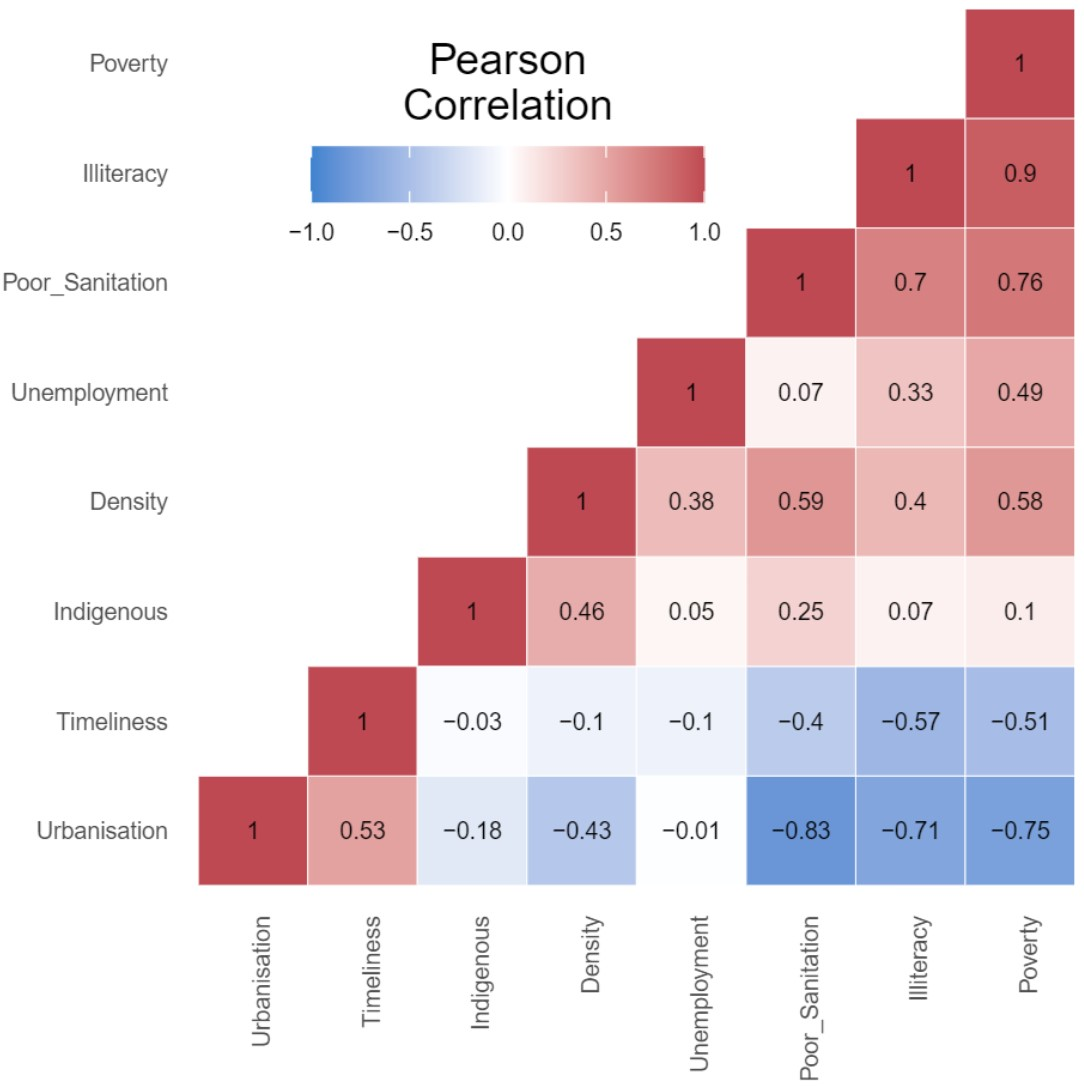
\includegraphics[scale=0.5]{pearson_correl.jpg}
\caption{\label{fig:pearson_correl}Correlogram shows covariates with highest positive and negative correlations.}
\end{figure}

\subsection{Tables}

\begin{table}[H]
\centering
\begin{tabular}{l|r}
Item & Quantity \\\hline
Widgets & 42 \\
Gadgets & 13
\end{tabular}
\caption{\label{tab:widgets}An example table.}
\end{table}

\subsection{Code}
\begin{minted}[
frame=lines,
framesep=2mm,
baselinestretch=1.2,
bgcolor=LightGray,
fontsize=\footnotesize,
linenos
]{R}


# Load Data
load("C:/Users/soura/Documents/COMM511/group_coursework/datasets_project.RData")
# Import Libraries
library(mgcv) # required for GAM 

#fit poisson model with socio-economic variables
model_poisson <- gam(formula = TB ~ offset(log(Population)) + s(Indigenous)
+ s(Illiteracy) + s(Urbanisation) + s(Density) + s(Poverty) + s(Poor_Sanitation)
+ s(Unemployment) + s(Timeliness), 
data = TBdata, 
family = poisson(link = 'log')
)
#check summary
summary(model_poisson)
model_poisson$aic
par(mfrow = c(2,2),pch = 20)
gam.check(model_poisson)

# #add flexibility
# model_poisson.more.knots <- gam(formula = TB ~ offset(log(Population)) + s(Indigenous, k = 60) 
# + s(Illiteracy, k = 60) +  s(Urbanisation, k = 60) + s(Density, k = 60) 
# + s(Poverty, k = 60) + s(Poor_Sanitation, k = 60) + s(Unemployment, k = 60) 
# + s(Timeliness, k = 60), 
# data = TBdata, 
# family = poisson(link = 'log')
# )
# 
# par(mfrow=c(2,2))
# gam.check(model_poisson.more.knots)
# summary(model_poisson.more.knots) # SIGNS OF OVERFIT
# par(mfrow=c(2,4))
# plot(model_poisson.more.knots) # SIGNS OF OVERFIT
# par(mfrow=c(2,2))

#fit negative binomial model with  socioeconomic
model_nb <- gam(formula = TB ~ offset(log(Population)) + s(Indigenous) 
+  s(Illiteracy) + s(Urbanisation) + s(Density) + s(Poverty) + s(Poor_Sanitation)
+ s(Unemployment) + s(Timeliness), 
data = TBdata, family = nb(link = 'log')
)
#Show summary
summary(model_nb)
model_nb$aic


#fit a linear relation between squared residuals and prediction to see whether another model describes the variance-fitted values relation better
summary(lm(log(model_nb$residuals^2) ~ log(predict(model_nb, type = 'response'))))

#drop Illiteracy
model_nb_2 <- gam(formula = TB ~ offset(log(Population)) + s(Indigenous) +  s(Urbanisation) + s(Density) 
+ s(Poverty) + s(Poor_Sanitation) + s(Unemployment) + s(Timeliness),
data = TBdata,
family = nb(link = 'log')
)

# Likelihood ratio test
anova.gam(model_nb_2, model_nb, test = 'F') # p-value is over 0.05
# The models are statistically indistinguishable

model_nb_3 <- gam(formula = TB ~ offset(log(Population)) + s(Indigenous) +  s(Urbanisation) + s(Density) 
+ s(Poor_Sanitation) + s(Unemployment) + s(Timeliness), 
data = TBdata, 
family = nb(link = 'log')
)
#LRT
anova.gam(model_nb_3, model_nb_2, test = 'F')# p-value is less than 0.05
# The models are statistically different. Poverty should not be excluded.

### Model chosen (with socio-economic covariates) is the negative binomial without Illiteracy
### as the effect of illiteracy cannot be reliably stated to be non-zero
summary(model_nb_2)# Only 44% of the deviance is explained. Adding temporal
# and spatial covariates may improve this
par(mfrow=c(2,2))
gam.check(model_nb_2)

### Increasing the knots to 20 yields minor improvement - discarded
prelim.model.4 <- gam(formula = TB ~ offset(log(Population)) + s(Indigenous , k = 20) 
+ s(Urbanisation , k = 20) + s(Density , k = 20) + s(Poverty , k = 20)
+ s(Poor_Sanitation , k = 20) + s(Unemployment , k = 20) + s(Timeliness , k = 20),
data = TBdata ,
family = nb(link = 'log')
)
# Show summary
summary(prelim.model.4)
par(mfrow=c(2,2))
gam.check(prelim.model.4)

#### Introducing temporality as a grouping variable
#Temporal model
par(mfrow = c(2,2), pch = 20)
model_nb_time <- gam(formula = TB ~ offset(log(Population)) + s(Indigenous, by = Year) 
+ s(Urbanisation, by = Year) + s(Density, by = Year) + s(Poverty, by = Year) + s(Poor_Sanitation, by = Year) 
+ s(Unemployment, by = Year) + s(Timeliness, by = Year), 
data = TBdata, 
family = nb(link = 'log')
)
# Show summary
summary(model_nb_time)
model_nb_time$aic

#### Temporality as a covariate
TBdata$Year.asFactor <- factor(TBdata$Year)

temporal.model <- gam(formula = TB ~ offset(log(Population)) + s(Indigenous)
+ s(Urbanisation) + s(Density) + s(Poor_Sanitation) + s(Unemployment) + s(Poverty)
+ s(Timeliness) + Year.asFactor,
data = TBdata ,
family = nb(link = 'log')
)
# Check summary
summary(temporal.model) # Temporal alone doesn't add much to explaining the variance

par(mfrow=c(2,2))
gam.check(temporal.model)
par(mfrow = c(1,1))

### Adding spatial covariates
spatial.model <- gam(formula = TB ~ offset(log(Population)) + s(Indigenous) 
+ s(Urbanisation) + s(Density) + s(Poor_Sanitation) + s(Unemployment) +s(Poverty)
+ s(Timeliness) + s(lon , lat),
data = TBdata , 
family = nb(link = 'log')
)
# Check summary
summary(spatial.model)

par(mfrow=c(2,2))
gam.check(spatial.model)
par(mfrow = c(1,1))
spatial.model$aic

### Using separate smoothers
spatial.model.2 <- gam(formula = TB ~ offset(log(Population)) + s(Indigenous) 
+ s(Urbanisation) + s(Density) + s(Poor_Sanitation) + s(Unemployment) + s(Poverty)
+ s(Timeliness) + te(lon , lat , k = 20),
data = TBdata , 
family = nb(link = 'log')
)
# Check summary
summary(spatial.model.2)

spatial.model.2$aic
par(mfrow=c(2,2))
gam.check(spatial.model.2 , pch = 20)
par(mfrow = c(1,1))

# Check if this model is significantly different from one with only socio-economic covariates
anova.gam(spatial.model.2, model_nb_2, test = 'LRT')

#### Spatio-temporal model
spatio.temporal.model <- gam(formula = TB ~ offset(log(Population)) + s(Urbanisation, by = Year.asFactor) 
+ s(Density, by = Year.asFactor) + s(Poverty, by = Year.asFactor) 
+ s(Poor_Sanitation, by = Year.asFactor) + s(Timeliness, by = Year.asFactor) 
+ s(Unemployment, by = Year.asFactor) + te(lon,lat, by = Year.asFactor), data = TBdata, family = nb(link = 'log'))
summary(spatio.temporal.model)
spatio.temporal.model$aic
gam.check(spatio.temporal.model)

### Spatio-temporal model (with Year as parametric covariate)
spatio.temporal.model.2 <- gam(formula = TB ~ offset(log(Population)) + s(Indigenous) 
+ s(Urbanisation) + s(Density) + s(Poor_Sanitation) + s(Unemployment) + s(Poverty)
+ s(Timeliness) + te(lon , lat , k = 20) + Year.asFactor,
data = TBdata , 
family = nb(link = 'log')
)
# Check summary
summary(spatio.temporal.model.2) # Temporal dimension as a parametric variable explains 
# slightly more of the deviance
spatio.temporal.model.2$aic
gam.check(spatio.temporal.model.2 , pch = 20)

\end{minted}


\subsection{Code Outputs}
\begin{minted}[
frame=lines,
framesep=2mm,
baselinestretch=1.2,
bgcolor=LightGray,
fontsize=\footnotesize,
linenos
]{R}

\end{minted}